\documentclass[a4paper,12pt]{article}
\usepackage[utf8]{inputenc}
\usepackage[T1]{fontenc}
\usepackage{lipsum} 
\usepackage{enumitem} % pa las listass
\usepackage{geometry} % pa los margene
\usepackage{graphicx} % pa las imagenes

\geometry{margin=2.5cm}

\title{Unidad Didáctica 1. Arranque y procesos del sistema}
\author{Alvaro Vazquez Vazquez}
\date{\today}


% Bloques de codigo

\usepackage{listings}
\usepackage{xcolor}

\lstset{
    basicstyle=\ttfamily,
    keywordstyle=\color{blue},
    stringstyle=\color{red},
    commentstyle=\color{green},
    showstringspaces=false,
    numbers=left,
    numberstyle=\tiny,
    frame=single,
    breaklines=true
    morekeywords={firefox, ls, cd, echo} 
}



% Inicio del documento

\begin{document}

\maketitle

\noindent
I.E.S. Fernando Aguilar Quignon \\
C/Conil de la Frontera, 3 \\
CP 11010, Cádiz \\
\hrule

\section*{Administración de Sistemas Operativos - 1a Evaluación (RA 2 – CE d, e, f)
Unidad Didáctica 1. Arranque y procesos del sistema}
Realiza en GNU/Linux los siguientes ejercicios:

\begin{enumerate}[label=\textbf{Pregunta \arabic*.}]
    \item Lanza el comando ps, que muestra los procesos del usuario en el shell actual.
    Ejecuta también el comando ps aux | less, que muestra de forma paginada todos los
    procesos existentes en el sistema. Investiga sobre los datos mostrados (columnas)
    y explica qué indica cada uno.

    \textbf{Respuesta:}

    \begin{figure}[h!]
        \centering
        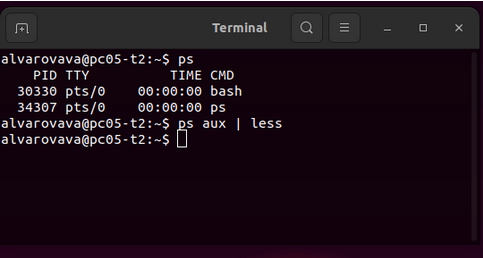
\includegraphics[width=0.7\textwidth]{1.png}
        \caption{Salida del comando ps.}
    \end{figure}
    \newpage
    \begin{figure}[h!]
        \centering
        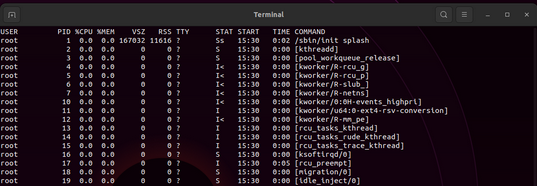
\includegraphics[width=0.7\textwidth]{2.png}
        \caption{Salida del comando ps aux.}
    \end{figure}



    Cuando lanzamos el comando \texttt{ps aux | less} se nos está ofreciendo información sobre los procesos. 
    El comando \texttt{ps} nos muestra todos los procesos que estén asociados al usuario y la terminal actual. 
    Muestra los campos básicos: 

    \begin{itemize}
        \item \textbf{PID}: Identificador del proceso.
        \item \textbf{TTY}: Terminal a la que está asociado el proceso.
        \item \textbf{TIME}: Tiempo de CPU acumulado.
        \item \textbf{CMD}: Comando que ha iniciado el proceso.
    \end{itemize}

    Por otro lado, al añadir las opciones \texttt{aux}: 
    \begin{itemize}
        \item \texttt{a}: Muestra todos los procesos con terminal asociada.
        \item \texttt{x}: Elimina la restricción de mostrar solo procesos con terminal asociada.
        \item \texttt{u}: Presenta la salida en un formato orientado a usuarios.
    \end{itemize}

    La salida incluye más campos, que indican lo siguiente:

    \begin{itemize}
        \item \textbf{USER}: Usuario propietario del proceso.
        \item \textbf{\%CPU}: Porcentaje de CPU que consume el proceso.
        \item \textbf{\%MEM}: Porcentaje de memoria principal (RAM) consumida.
        \item \textbf{STAT}: Estado del proceso y modificadores 
        (por ejemplo, \texttt{>} alta prioridad, \texttt{N} baja prioridad).
        \item \textbf{START}: Hora o fecha de inicio del proceso 
        (hora si es reciente, fecha si es antiguo).
        \item \textbf{VSZ}: Tamaño virtual del proceso en memoria (KB), 
        incluyendo código, datos y librerías compartidas.
        \item \textbf{RSS}: Resident Set Size, memoria física real (RAM) ocupada por el proceso (KB).
    \end{itemize}


    \newpage
    \item Ejecuta el comando ps axo pid,cmd,pri,nice | less, que muestra las columnas PID,
    CMD, PRI (prioridad) y NI (nice) de todos los procesos que existen actualmente en
    el sistema. ¿Qué indica la columna PRI y NI? Investiga para responder a la pregunta.


    \textbf{Respuesta:}


    \begin{figure}[h!]
        \centering
        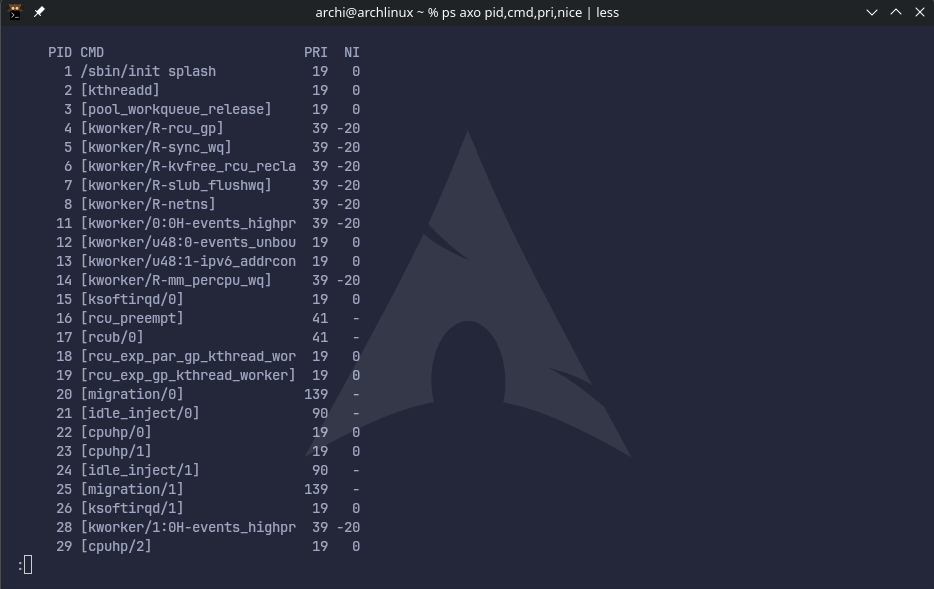
\includegraphics[width=0.7\textwidth]{3.png}
        \caption{Salida del comando ps axo pid,cmd,pri,nice.}
    \end{figure}
    \begin{itemize}
         
    
    \item La columna \textbf{PID} muestra el id de los procesos
    \item \textbf{CMD} muestra el comando que lanza dicho proceso.
    \item \textbf{PRI} muestra la prioridad del proceso que ua el planificador de linux para decidir qué proceso ejecutar primero. Cuanto mas bajo sea este numero, mas prioridad tiene. Estos numeros pueden variar entre 0 y 139.
    \item La columna \textbf{NI} muestra el valor de "niceness" del proceso, que va de -20 a 19 e indica la prioridad relativa del proceso. Valores más bajos (-20) significan mayor prioridad, mientras que valores más altos (+19) indican menor prioridad. El valor por defecto es 0. Los usuarios normales no pueden asignar valores negativos; solo el superusuario puede hacerlo. Este valor es utilizado por el planificador de Linux para ajustar la prioridad del proceso (PRI) en función de su "niceness". Un proceso con un valor de NI más bajo tendrá una prioridad (PRI) más alta, lo que significa que es más probable que sea seleccionado para la ejecución antes que otros procesos con valores de NI más altos.
    
    \end{itemize}
    \newpage
    \item Teniendo en cuenta lo anterior, lanza el comando TOP y comenta la relación entre la columna PR y NI. ¿Es similar la columna PRI a PR?

    \textbf{Respuesta:}
    
    La columna \textbf{PRI} del comando anterior y la columna \textbf{PR} del comando \texttt{top} están relacionadas, pero no son exactamente lo mismo. PR es la representacion en tiempo real de la prioridad del proceso, como lo ve top. Muestra el mismo valor que PRI, pero a menudo se redondea para que sea mas legible.

    Por otro lado la columna NI de top y NI de ps axo son exactamente iguales y sus campos han sido explicados anteriormente.

    \begin{figure}[h!]
        \centering
        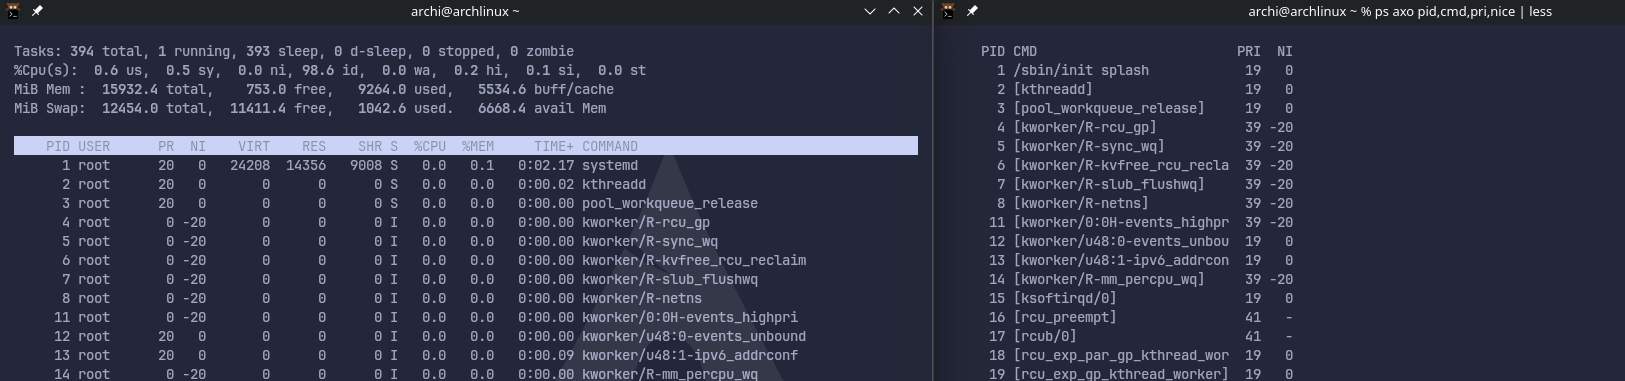
\includegraphics[width=0.7\textwidth]{4.png}
        \caption{Salida del comando ps axo pid,cmd,pri,nice.}
    \end{figure}

    \item Explica cómo utilizar el comando pstree. Se tratarán todos los detalles vistos
    durante las sesiones de clase.

    \textbf{Respuesta:} 

    RESPONDER


    \item Detalla cómo utilizar el comando top. En la explicación deberán aparecer todos los aspectos explicados en clase.

    \textbf{Respuesta:}
    
    Esta herramienta proporciona una vista en tiempo real de los procesos en ejecución y el uso de recursos del sistema. 

    
    Podemos lanzar la herramienta con la opcion -o USER para filtrar por usuario. con la opcion -o PID podemos filtrar por PID. Tambien podemos usar la opcion -n para indicar el numero de actualizaciones que queremos ver antes de que top se cierre automaticamente. Pero dentro de la herramienta podemos usar varios comandos para interactuar con ella:
    

    % He estado un rato jugando con la herramienta


    \begin{itemize}
        \item \textbf{h}: Muestra la ayuda con todos los comandos disponibles.
        \item \textbf{q}: Sale de la herramienta top.
        \item \textbf{P}: Ordena los procesos por uso de CPU (de mayor a menor).
        \item \textbf{M}: Ordena los procesos por uso de memoria (de mayor a menor).
        \item \textbf{T}: Ordena los procesos por tiempo de ejecución (de mayor a menor).
        \item \textbf{k}: Permite matar un proceso. Se te pedirá el PID del proceso que deseas terminar.
        \item \textbf{r}: Cambia la prioridad (renice) de un proceso. Se te pedirá el PID y el nuevo valor de nice.
        \item \textbf{1}: Muestra o oculta el desglose del uso de CPU por núcleo.
        \item \textbf{s} Cambia el intervalo de actualización en segundos.
        \item \textbf{o} Permite ordenar los procesos por cualquier columna. Se te pedirá que ingreses el nombre de la columna.
        
    \end{itemize}

    \textbf{Nota:} Algunas teclas tienen funciones distintas según se pulsen en minúscula o en mayúscula.




    \item Documenta cómo gestionar los procesos del sistema utilizando los comandos kill,
    jobs, fg y bg.

    \textbf{Respuesta:}

    \begin{figure}[h!]
        \centering
        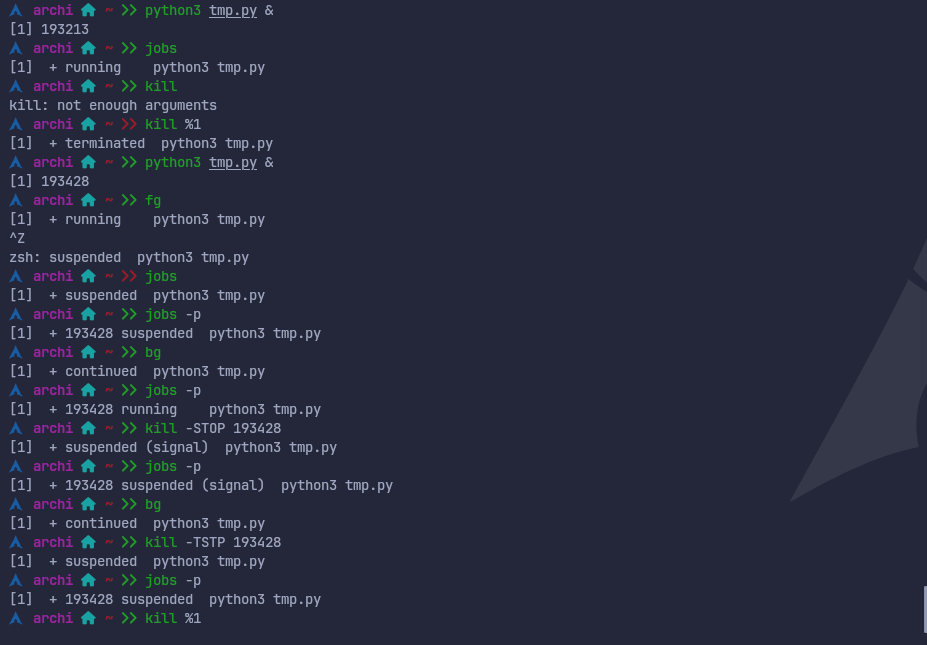
\includegraphics[width=0.7\textwidth]{5.png}
        \caption{Gestionando procesos con fg,bg y jobs.}
    \end{figure}

    Con jobs he visto que trabajos están en segundo plano.
    En este caso estaba en estado running. He intentado mandarle un SIGTERM con kill, pero no ha detectado automaticamente que me estoy refiriendo al primer (y unico) argumento o trabajo. Por lo que le he tenido que mandar el parametro \%1.
    Luego con fg he traido el proceso a primer plano y con ctrl + z le he mandado un SIGTSTP. Al lanzar jobs se aprecia como esta en estado suspended. Con jobs -p he visto el PID del proceso, con bg le he mandado a segundo plano y un SIGCONT. El proceso esta en estado running de nuevo. Esta vez sabiendo su PID gracias a jobs -p le he mandado un kill -STOP -PID-. Y luego un kill -TSTP -PID-.


    \item \texttt{Analizar el funcionamiento de la herramienta gráfica Monitor de sistema (gnome-system-monitor) proporcionada por el entorno de escritorio GNOME. La herramienta permite, entre otras cosas, monitorizar y gestionar los procesos, asi como observar un histórico de uso de la/s CPU/s.}
    
    \textbf{Respuesta:}

    Esta herramienta es una interfaz gráfica que permite a los usuarios monitorizar y gestionar los procesos del sistema de manera visual e intuitiva. Proporciona una vista en tiempo real del uso de recursos del sistema, incluyendo CPU, memoria, disco y red.


\end{enumerate}
\end{document}


